\section{Network Architecture and Methodology}
\subsection{Unet}
%TODO describe Unet here
\begin{table}
\centering
	\begin{tabular}{l c c c}
	\hline
	\hline
	Layer	&	input	&	output	&	channel	\\
	\hline
	Conv 3x3 + RELU	&	572	&	570	&	64	\\
	Conv 3x3 + RELU	&	570	&	568	&	64	\\
	Max Pool 2 $\times$ 2	&	568	&	284	&	64	\\
	Conv 3x3 + RELU	&	284	&	282	&	128	\\
	Conv 3x3 + RELU	&	282	&	280	&	128	\\
	Max Pool 2 $\times$ 2	&	280	&	140	&	128	\\
	Conv 3x3 + RELU	&	140	&	138	&	256	\\
	Conv 3x3 + RELU	&	138	&	136	&	256	\\
	Max Pool 2 $\times$ 2	&	136	&	68	&	256	\\
	Conv 3x3 + RELU	&	68	&	66	&	512	\\
	Conv 3x3 + RELU	&	66	&	64	&	512	\\
	Max Pool 2 $\times$ 2	&	64	&	32	&	512	\\
	Conv 3x3 + RELU	&	32	&	30	&	1024	\\
	Conv 3x3 + RELU	&	30	&	28	&	1024	\\
	up-conv 2 $\times$ 2	&	28	&	56	&	512	\\
	convs 1x1	&	56	&	54	&	512	\\
	convs 1x1	&	54	&	52	&	512	\\
	up-conv 2 $\times$ 2	&	52	&	104	&	256	\\
	convs 1x1	&	104	&	102	&	256	\\
	convs 1x1	&	102	&	100	&	256	\\
	up-conv 2 $\times$ 2	&	100	&	200	&	128	\\
	convs 1x1	&	200	&	198	&	128	\\
	convs 1x1	&	198	&	196	&	128	\\
	up-conv 2 $\times$ 2	&	196	&	392	&	64	\\
	convs 1x1	&	392	&	390	&	64	\\
	convs 1x1	&	388	&	388	&	2	\\
	\hline
	\hline
	\end{tabular}
	\caption{The Original Unet Architechture}
	\label{tab:OriginalUnet}
\end{table}
\subsection{Attention Gate}
%TODO Describe Attention gate here
\section{presenting with unlabelled data}
\subsection{Psuedo labeling}
\subsection{Semi-supervise architecture}
As we described in Chapter 2, we designed a Mean-teacher style model for the semi-supervise task.
\begin{figure}
	\centering
	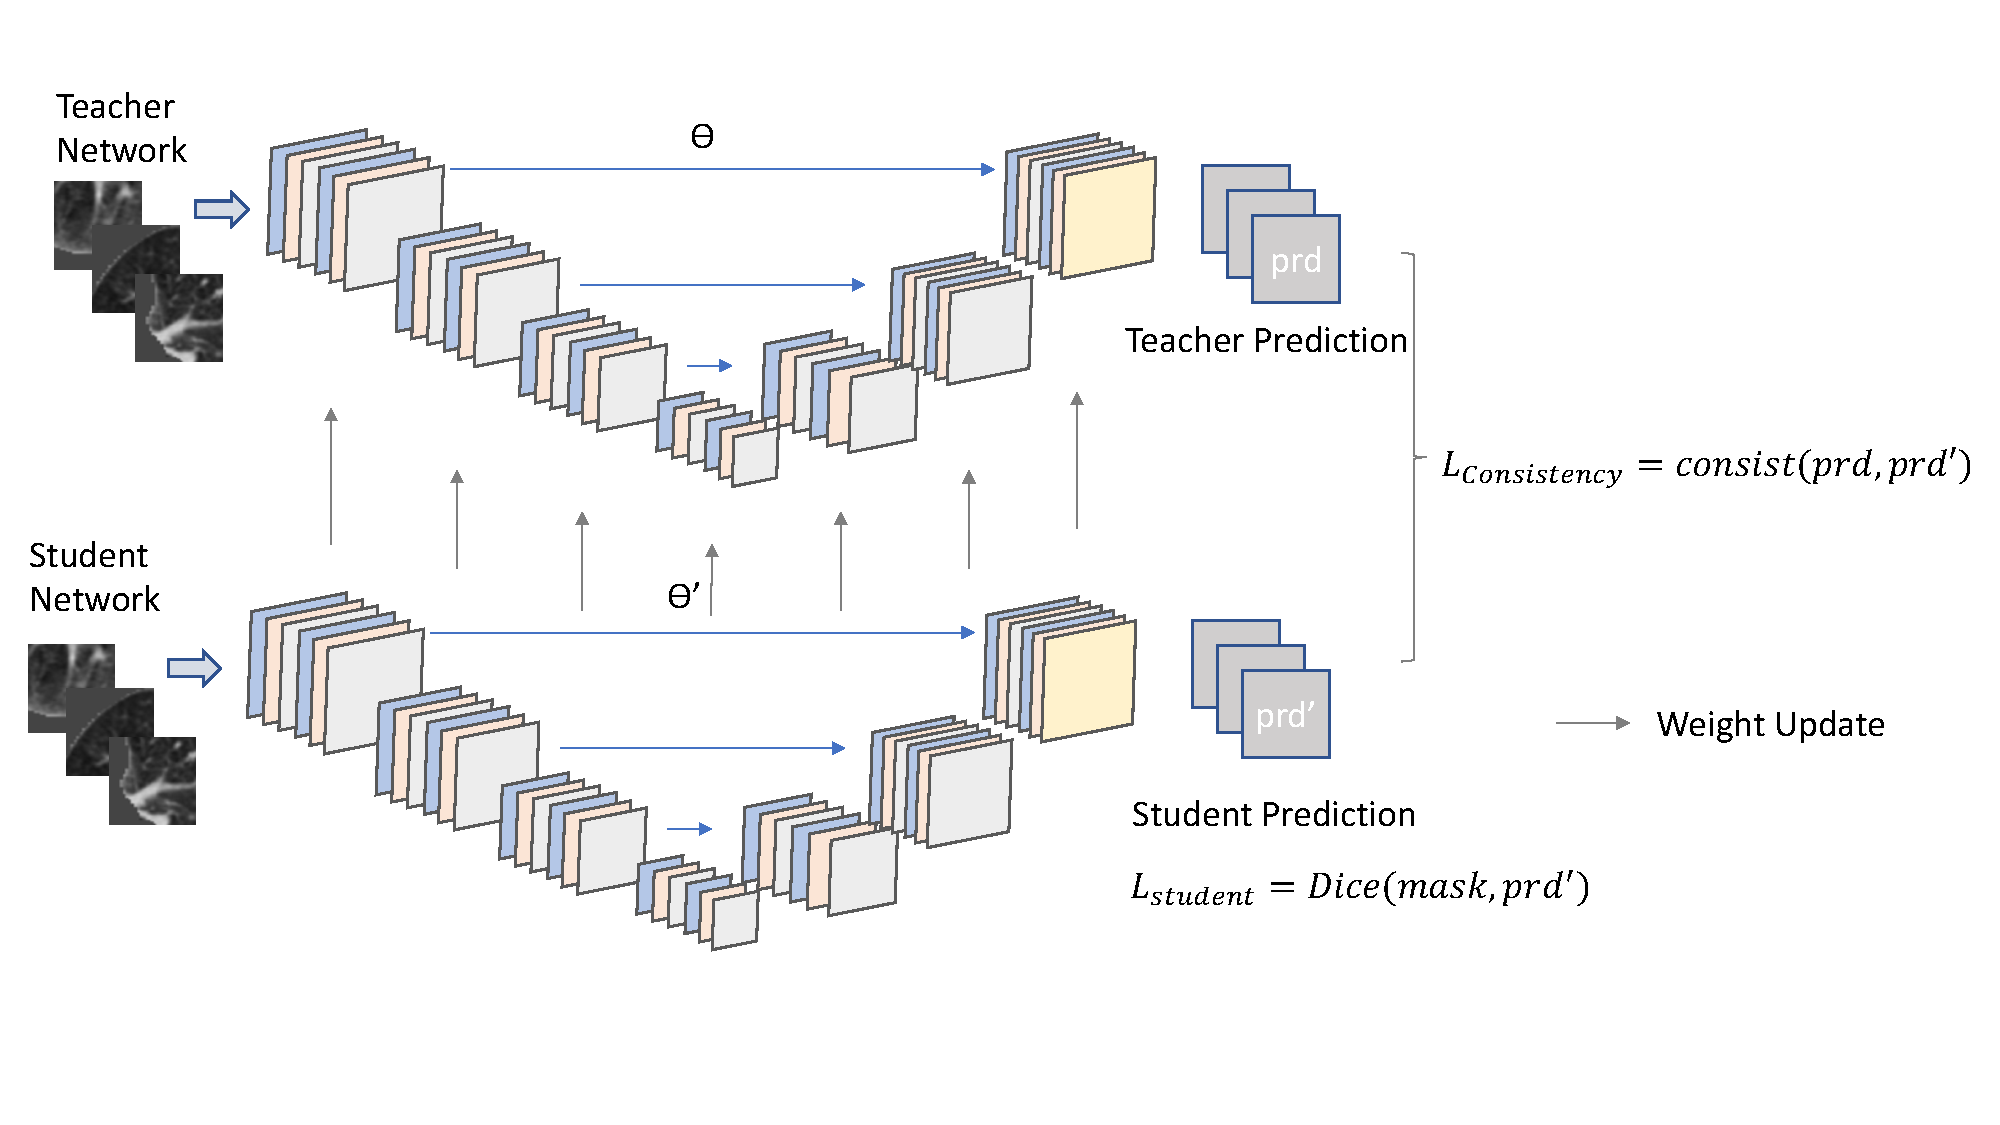
\includegraphics[width=0.8\textwidth]{img/Networks/mean-teacher-net}
	\caption{The design of network model for our semi-supervise setup}
\end{figure}